\documentclass[a4paper]{article}

%% Language and font encodings
\usepackage[english,spanish]{babel}
\usepackage[utf8x]{inputenc}
\usepackage[T1]{fontenc}

\usepackage{hyperref}
\usepackage{caption}
\usepackage{subcaption}
\usepackage{booktabs}

%% Sets page size and margins
\usepackage[a4paper,top=3cm,bottom=2cm,left=3cm,right=3cm,marginparwidth=1.75cm]{geometry}

%% Useful packages
\usepackage{amsmath}
\usepackage{graphicx}
\usepackage[colorinlistoftodos]{todonotes}

\begin{document}

\title{%

\includegraphics[scale = 0.5]{./header_unc.png}\\[1.0 cm]	% University Logo
  Arquitectura de Computadoras \\
  \large Ingeniería en Computación FCEFyN - UNC\\
  		Trabajo Práctico 2 - UART
  }


  \author{Izquierdo Agustina Mat: 37729473\\
          Salvatierra Andrés Mat: 39611008}
  
  \date{22 de octubre de 2019}
\maketitle
\newpage

\section{Introducción}
Para el segundo trabajo práctico de la materia se realizó la implementación en Verilog de un módulo UART. 
El mismo se desarrolló para la placa Basys 3 utilizando el software Vivado 2018.2.
El módulo se conecta a la ALU, desarrollada en el primer práctico, y a una PC desde la cual es posible enviar los parámetros(mediante un script en python) necesarios para que la unidad aritmética procese.

\begin{figure}[!htb]
\centering
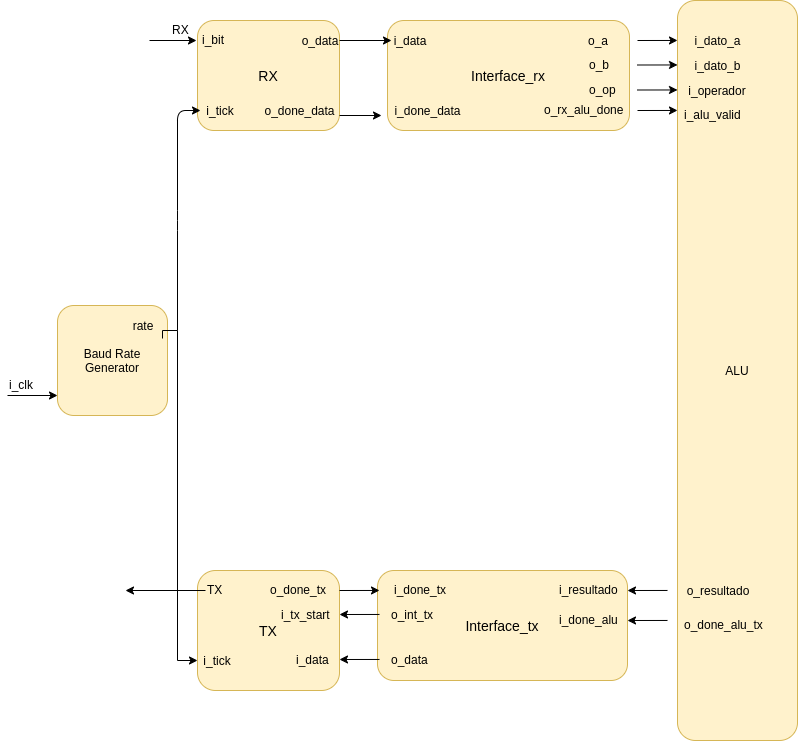
\includegraphics[width=.95\textwidth]{bloque_gral.png}
\caption{\label{fig:tp2_uart}Diagrama de bloque general}
\end{figure}

\newpage

\section{Desarrollo}

Se definió un módulo top\_gral, el cual contiene:
    \begin{itemize}
        \item Módulo UART
            \begin{itemize}
            \item tx 
            \item rx
            \item baudrate\_gen
            \end{itemize}
        \item Módulo interfaz\_tx
        \item Módulo interfaz\_rx
        \item Módulo ALU
    \end{itemize}

\subsection{Módulo UART}
\subsubsection{Módulo baudrate\_gen}
Este módulo es utilizado para generar una señal de muestreo para el modulo RX y TX. Generando un tick 16 veces por Baud Rate.
A partir de la entrada de clock (conociendo su frecuencia) y la velocidad de transmisión de la UART (en este caso, 9600 baudios), genera ticks que permiten al módulo Rx trabajar con la señal de entrada y al Tx con la señal de salida.

\subsubsection{Módulo tx}
Es una máquina de estados que utiliza la señal proveniente del BaudRate Generador para actualizar su salida (Tx) acorde a la información que
se desea transmitir. Al finalizar la transmisión emite un pulso en una señal de fin (tx\_done\_tick) notificándole a la interfaz\_tx

Inicia en el estado IDLE, en el que envía por Tx un 1 lógico (canal inactivo). Al recibir la señal i\_tx\_start (proveniente de la interfaz\_tx) pasa al estado START, en el que se envía un 0 lógico por el canal durante 16 ticks del Baud Rate Generator.
A continuación se pasa al estado DATA, en el que se envía por 16 ticks cada bit del byte a transmitir, comenzando por el menos significativo. Cuando la cantidad de bits enviados sea 8 (toda la información disponible), se pasa al estado STOP, en el que se envia un bit de stop por 16 ticks del Generator. En este estado se le notifica a la interfaz\_tx que el dato ya fue transmitido y puede recibir uno nuevo.
Finalmente se pasa al estado IDLE nuevamente, a la espera de más bits para transmitir.


\begin{figure}[!htb]
\centering
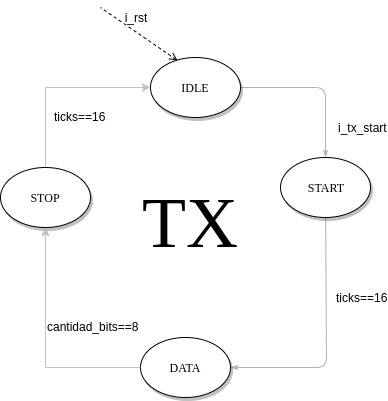
\includegraphics[width=0.4\textwidth]{tx_tp2.jpeg}
\caption{\label{fig:tests}Diagrama de estados del transmisor}
\end{figure}

\subsubsection{Módulo rx}
Es una máquina de estados que modifica su comportamiento en función de la entrada proveniente de la PC y el modulo Generador de Baudrate. 

Inicia en el estado IDLE, hasta que la entrada sea un 0 logico, lo que marca el inicio (i\_start) del bit de start. Luego de esto pasa al estado START, que espera 7 ticks hasta situarse en el centro del bit de start (que dura 16 ticks), lo que sincroniza el módulo con el transmisor. En consecuencia, se pasa al estado DATA, en el que toma muestras cada 16 ticks, que marcan el centro de cada bit recibido. El paso siguiente es pasar al estado STOP, donde se lee el único bit de stop, y finalmente se pasa al estado IDLE para comenzar el ciclo nuevamente. Al finalizar la recepción de un valor, emite un pulso(o\_done\_data), indicándole a la interfaz que hay un nuevo dato.

\begin{figure}[!htb]
\centering
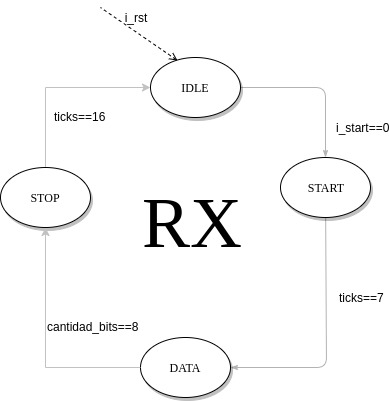
\includegraphics[width=0.4\textwidth]{rx_tp2.jpeg}
\caption{\label{fig:tests}Diagrama de estados del Receptor}
\end{figure}

\subsection{Módulo interfaz transmisor}
Permite comunicar la ALU con el modulo TX del UART.

Inicia en el estado IDLE hasta que la ALU le notifica (i\_done\_data) que tiene el resultado de una operación. Luego de esto pasa al estado ALMACENAR, cuando el modulo TX le notifica a la interfaz (i\_done\_tx) que esta libre y puede transmitir un dato pasa al estado PUSH ON donde transmite el dato y por último vuelve al estado inicial.
\begin{figure}[!htb]
\centering
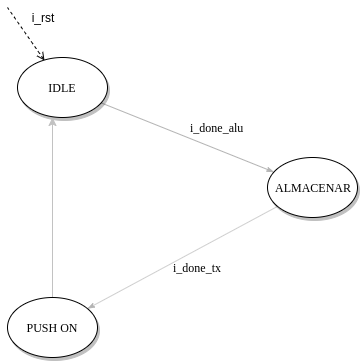
\includegraphics[width=0.4\textwidth]{int_tx.png}
\caption{\label{fig:tests}Diagrama de estados de la interfaz del transmisor}
\end{figure}

\newpage

\subsection{Módulo interfaz receptor}
Permite comunicar la ALU con el modulo RX del UART. Es una máquina de estados que modifica su comportamiento en función de la entrada proveniente del RX.

Inicia en el estado IDLE hasta que el modulo RX le notifica (i\_done\_data) que tiene un dato. Luego de esto pasa OP1 y sucede lo mismo hasta llegar al estado OPERACION. En este momento ya tenemos los 3 datos disponibles y pasa al estado ALU, aquí le notifica al modulo ALU que tiene los 3 datos listos para que este último modulo opere. Luego de esto vuelve al estado inicial.
\begin{figure}[!htb]
\centering
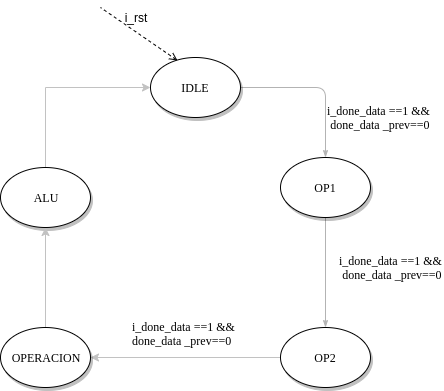
\includegraphics[width=0.4\textwidth]{int_rx.png}
\caption{\label{fig:tests}Diagrama de estados de la interfaz del receptor}
\end{figure}


\subsection{Módulo ALU}
El módulo ALU es el desarrollado en el primer práctico. Es puramente combinacional, con dos entradas para operandos, y una entrada para el operador.


\subsection{Verificación - Test Bench}
Se realizaron test bench para cada modulo del sistema. Entre los más destacados:

\subsubsection{Interface}
Permite verificar el comportamiento de ambas interfaces y la ALU. Simula la entrada de tres valores (operandos y operador), y permite ver que efectivamente son recibidos por la unidad aritmética generando un resultado que llega a la interface del TX.

\subsubsection{UART}
Comprueba el correcto funcionamiento del sistema. Se simuló el ingreso de 3 valores (uno correspondiente al dato A, otro al dato B y por último al operador) cada uno con su bit de inicio y stop.  Cada uno de estos datos es procesado por el bloque RX y pasa por la interfaz\_rx. Cuando ingresa el tercer dato, estos valores ingresan a la ALU, se realiza la operación correspondiente y el resultado de la misma pasa por la interfaz\_tx y sale por el bloque TX a la computadora(script python).
Esto se puede ver en la siguiente figura. Cables:
\begin{itemize}
\item rx\_interfaz\_done\_data: notifica a la interfaz que tiene un dato listo
\item rx\_interfaz\_data: dato
\item dato\_a: operando a
\item dato\_b: operando b
\item operador: operador
\item rx\_alu\_done: notifica ALU que tiene los 3 datos
\item done\_alu\_tx: ALU notifica al tx que tiene el resultado
\item resultado: resultado de la operación
\end{itemize}
\begin{figure}[!htb]
\centering
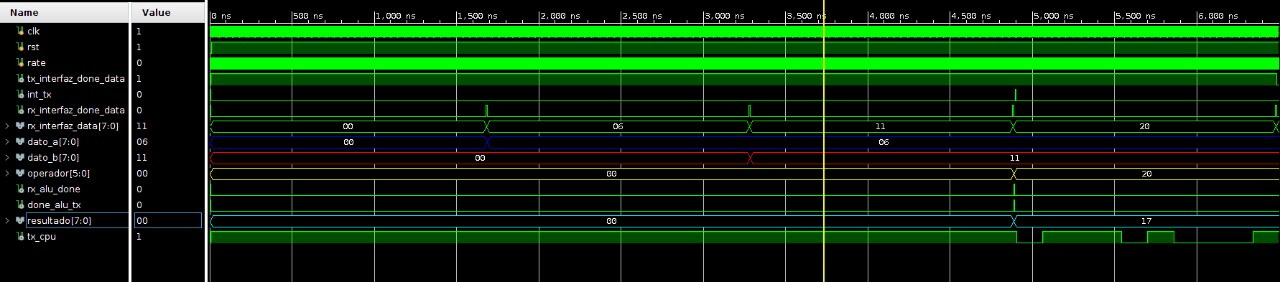
\includegraphics[width=1\textwidth]{Tb_uart.jpeg}
\caption{\label{fig:tests}Test Bench Uart}
\end{figure}

\subsection{Interfaz con la PC}
Para probar el funcionamiento de todo el proyecto, se programó un script en Python que se comunica con la FPGA mediante conexión USB, utilizando la librería PySerial.
\begin{figure}[!htb]
\centering
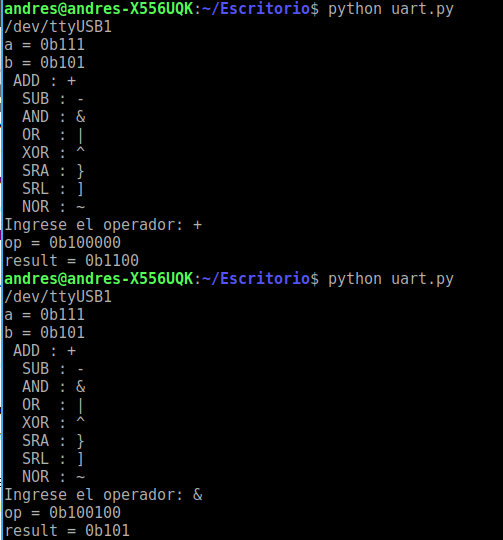
\includegraphics[width=0.5\textwidth]{resultado.png}
\caption{\label{fig:tests}Test Bench Uart}
\end{figure}
\end{document}